\documentclass{article}
\usepackage{enumitem}
\usepackage[cachedir=minted_cache]{minted}
\usepackage{graphicx}
\graphicspath{ {./img/} }
\usepackage[margin=1in]{geometry} %used to set the margins
\setcounter{secnumdepth}{0} %used to get rid of section numbers
\title{Lab 5 Selection}
\author{Michael Morikawa}
\date{\today}


\begin{document}
\maketitle
\section{Lab Questions}
\begin{enumerate}[label=\textbf{Question \arabic*}]
    \item Provide some good reasons that you might not want to sort the data in
          order to determine the median value.\\
          \textbf{You do not need to sort the data to get the median because it does extra work
              and for larger data sets it will be slow. You could partially sort but again for large data sets
              it would be a lot of work.}
    \item Explain how the prune-and-search design pattern works. Is recursion
          always necessary? Explain. \\
          \textbf{
              The prune-and-search design patter works by removing/pruning away  elements from
              the collection that we are working until we reach a set size. Once the size is reached
              the problem is solved using brute force. Recursion is not always necessary; you can
              sometimes iteratively reduce the elements you are working with. For example you do
              an iterative binary search which would fall under this category of algorithms.
          }

\end{enumerate}

\section{Source Code}
\subsection{main.cpp}
\inputminted{c++}{../src/main.cpp}
\section{Output}
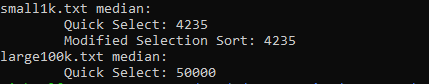
\includegraphics[]{output.png}

\end{document}